\chapter{Equipotential Curves}

\section*{Objectives}
\begin{enumerate}
\item To understand the relationship between electric fields and voltages.
\item To study the properties of electric fields in two-dimensions by mapping equipotential curves and constructing the corresponding lines of force.
\end{enumerate}


\section*{Introduction}

You may remember from school that any configuration of static electric charges produces an electric field in space. Such an electric field is a vector quantity that is a function of position, meaning that it has both a magnitude and direction at every point in space. Consider, for example, a point charge $q$ at the origin, whose electric field is well known from Coulomb's law,
\begin{equation}
    \vb{E} = \frac{1}{4\pi \epsilon_0} \frac{q}{r^2} \hat{\vb{r}}.
\end{equation}

The above equation tells us that the electric field vectors point radially outward\footnote{Or inward, if the charge is negative.} from the charge and that their magnitudes fall off as the reciprocal of the square of the distance from it.

When one has a collection of several charges, the electric field obeys the principle of superposition. In other words, the resulting electric field is the vector sum of all the contributions of the individual parts. This makes it possible to (theoretically) calculate the field produced by any collection of charges. Practically, however, this is very hard to do even for simple charge configurations, because of the vector nature of the field. This also results in the electric field being difficult to grasp or visualise. There is, however, a very simple way to arrive at this vector field, using a concept known as the \textsl{electric potential} $V$.

\section*{Theory}

\subsection*{Electric fields and potentials}

Maxwell's equations completely describe a static electric field through its divergence and curl
\begin{equation}
    \begin{aligned}
        \div{\vb{E}} &= \rho/\epsilon_0,\\
        \curl{\vb{E}}&= \vb{0},
    \end{aligned}
\end{equation}

where $\rho$ is the charge density and $\epsilon_0$ a constant known as the permittivity of free space.

\begin{question}
\textbf{Question:} Using the second equation above, show that this implies that every static electric field can be expressed as the gradient of a \textsl{scalar} field, called the electric potential $V$. In other words, show that 
\begin{equation}
    \vb{E} = - \gradient{V}
\end{equation}
\end{question}

If no net charge accumulates in a region, we can say that the charge density $\rho = 0$ in this region. In this case, the potential satisfies \textsl{Laplace's Equation}:
\begin{equation}
    \laplacian{V} = 0.
    \label{eqn:laplace}
\end{equation}

Being a scalar, $V$ just requires a single number at every point, which makes it much easier to work with. We can obtain the electric field from the potential by taking its \textsl{gradient}. The gradient of a scalar function is a vector whose $x$, $y$, and $z$ components are the rate at which the function changes along $x$, $y$, and $z$, respectively. A consequence of this is that the gradient vector, at any position, points along the direction in which function changes fastest and its magnitude is the rate of change of the function along this direction. Thus, the potential contains all the information that the field does.

Here is a simple way to visualise this: imagine connecting the points at which the potential has the same value. This is rather like connecting the points on a hill that are at the same height.\footnote{Or rather, same ``gravitational'' potential!} If this is done for a series of equally spaced values, what results is a contour map, with each contour representing a single value of the height. In the case of electric potential, these contours are called equipotential curves.\footnote{In general, in three dimensions, the points which have the same potential lie on a two-dimensional surface, known as an equipotential surface.} It is easy to see that where the contours are closely spaced the potential changes rapidly and where they are widely spaced the potential changes slowly in space. Given how the potential is defined (as a gradient), it should be easy to see that the magnitude of the electric field is larger in the first case than in the second case. Another important rule about these contour lines and the electric field is that field lines always meet contour lines at right angles. This is because the $\vb{E}$ field always points in the direction where $V$ is changing the most rapidly. It makes sense, then, that the direction perpendicular to the $\vb{E}$ field is the direction where $V$ is not changing at all. Since this direction must be along the equipotential surface by definition, the electric field is locally perpendicular to the equipotential surface.

\begin{question}
\textbf{Question:} What are the equipotential surfaces for the point charge we discussed earlier? Consider three equipotential surfaces that are equally spaced in potential. Are they spaced equally \textsl{in space}? If yes, why? If not, how do they change? How would this change if the charge was negative instead of positive?

\textbf{Question:} Now imagine an infinite wire of charge lying along the $x$-axis. What would the equipotential surfaces be in this case?
\end{question}

\subsection*{Conductors as equipotential surfaces}

A conductor is a material with the property that the charge in it is free to move around. A material which does not have this property (i.e.\ one in which the charges are stationary) is called an insulator. In practice, almost all metals are good conductors and most other substances are insulators. In static equilibrium has the property that the electric field is zero everywhere inside. The reason is simple: if it weren't zero somewhere, the charge there would move in the direction of the field, so it wouldn't be in static equilibrium. One important consequence of this is that all points within a conductor are at the same potential. This is because a difference in potential would imply an electric field, which would push the electrons in the conductor in such a way as to reduce the field; this continues until the electrons in the interior or the conductor are pushed to the surface. And, on the surface, they are moved around until the component of the field along it vanishes. Thus, the surface of a conductor is an equipotential surface.

\begin{imp}
Suppose now you have a region of space enclosed by two equipotential surfaces (say, the region between two concentric spheres), and you are interested in the potential at all points between them. We can compute the potential at every point in this region of space by solving Laplace's Equation (Equation~(\ref{eqn:laplace})) with the appropriate value at the boundaries. We can then find the equipotential surfaces, since they are simply are the loci of points where this solution to Laplace's Equation has the same value.
\end{imp}

% \begin{imp}
% Be careful about applying these facts too generally: it's very easy to have a conductor which is not in static equilibrium! This is why conductors are usually used: to maintain a steady flow of charge, what we call a current, as you will learn in another experiment. A conductor which is carrying a current is not an equipotential; instead, the current flows from high to low potential inside the conductor.
% \end{imp}

Since the conductors we will be using are equipotential surfaces, we can find the potential in the region in between them by solving Laplace's Equation. This is, in general, a daunting task. However we can often use the symmetry of simple configurations to solve for $V$ easily.

\subsection*{Some interesting configurations}

In this experiment, you will be given some metal electrodes and asked to find the curves of constant potential. You will be asked routinely to solve such problems in electrostatics in the course on \textsl{Electricity and Magnetism} you have this semester. Let us try to do this for some simple configurations. We will be working in two dimensions of space (the surface of the water). 

\begin{figure}[!htb]
\captionsetup[subfigure]{justification=centering}
\centering
        \begin{subfigure}[b]{0.6\textwidth}
        \centering
                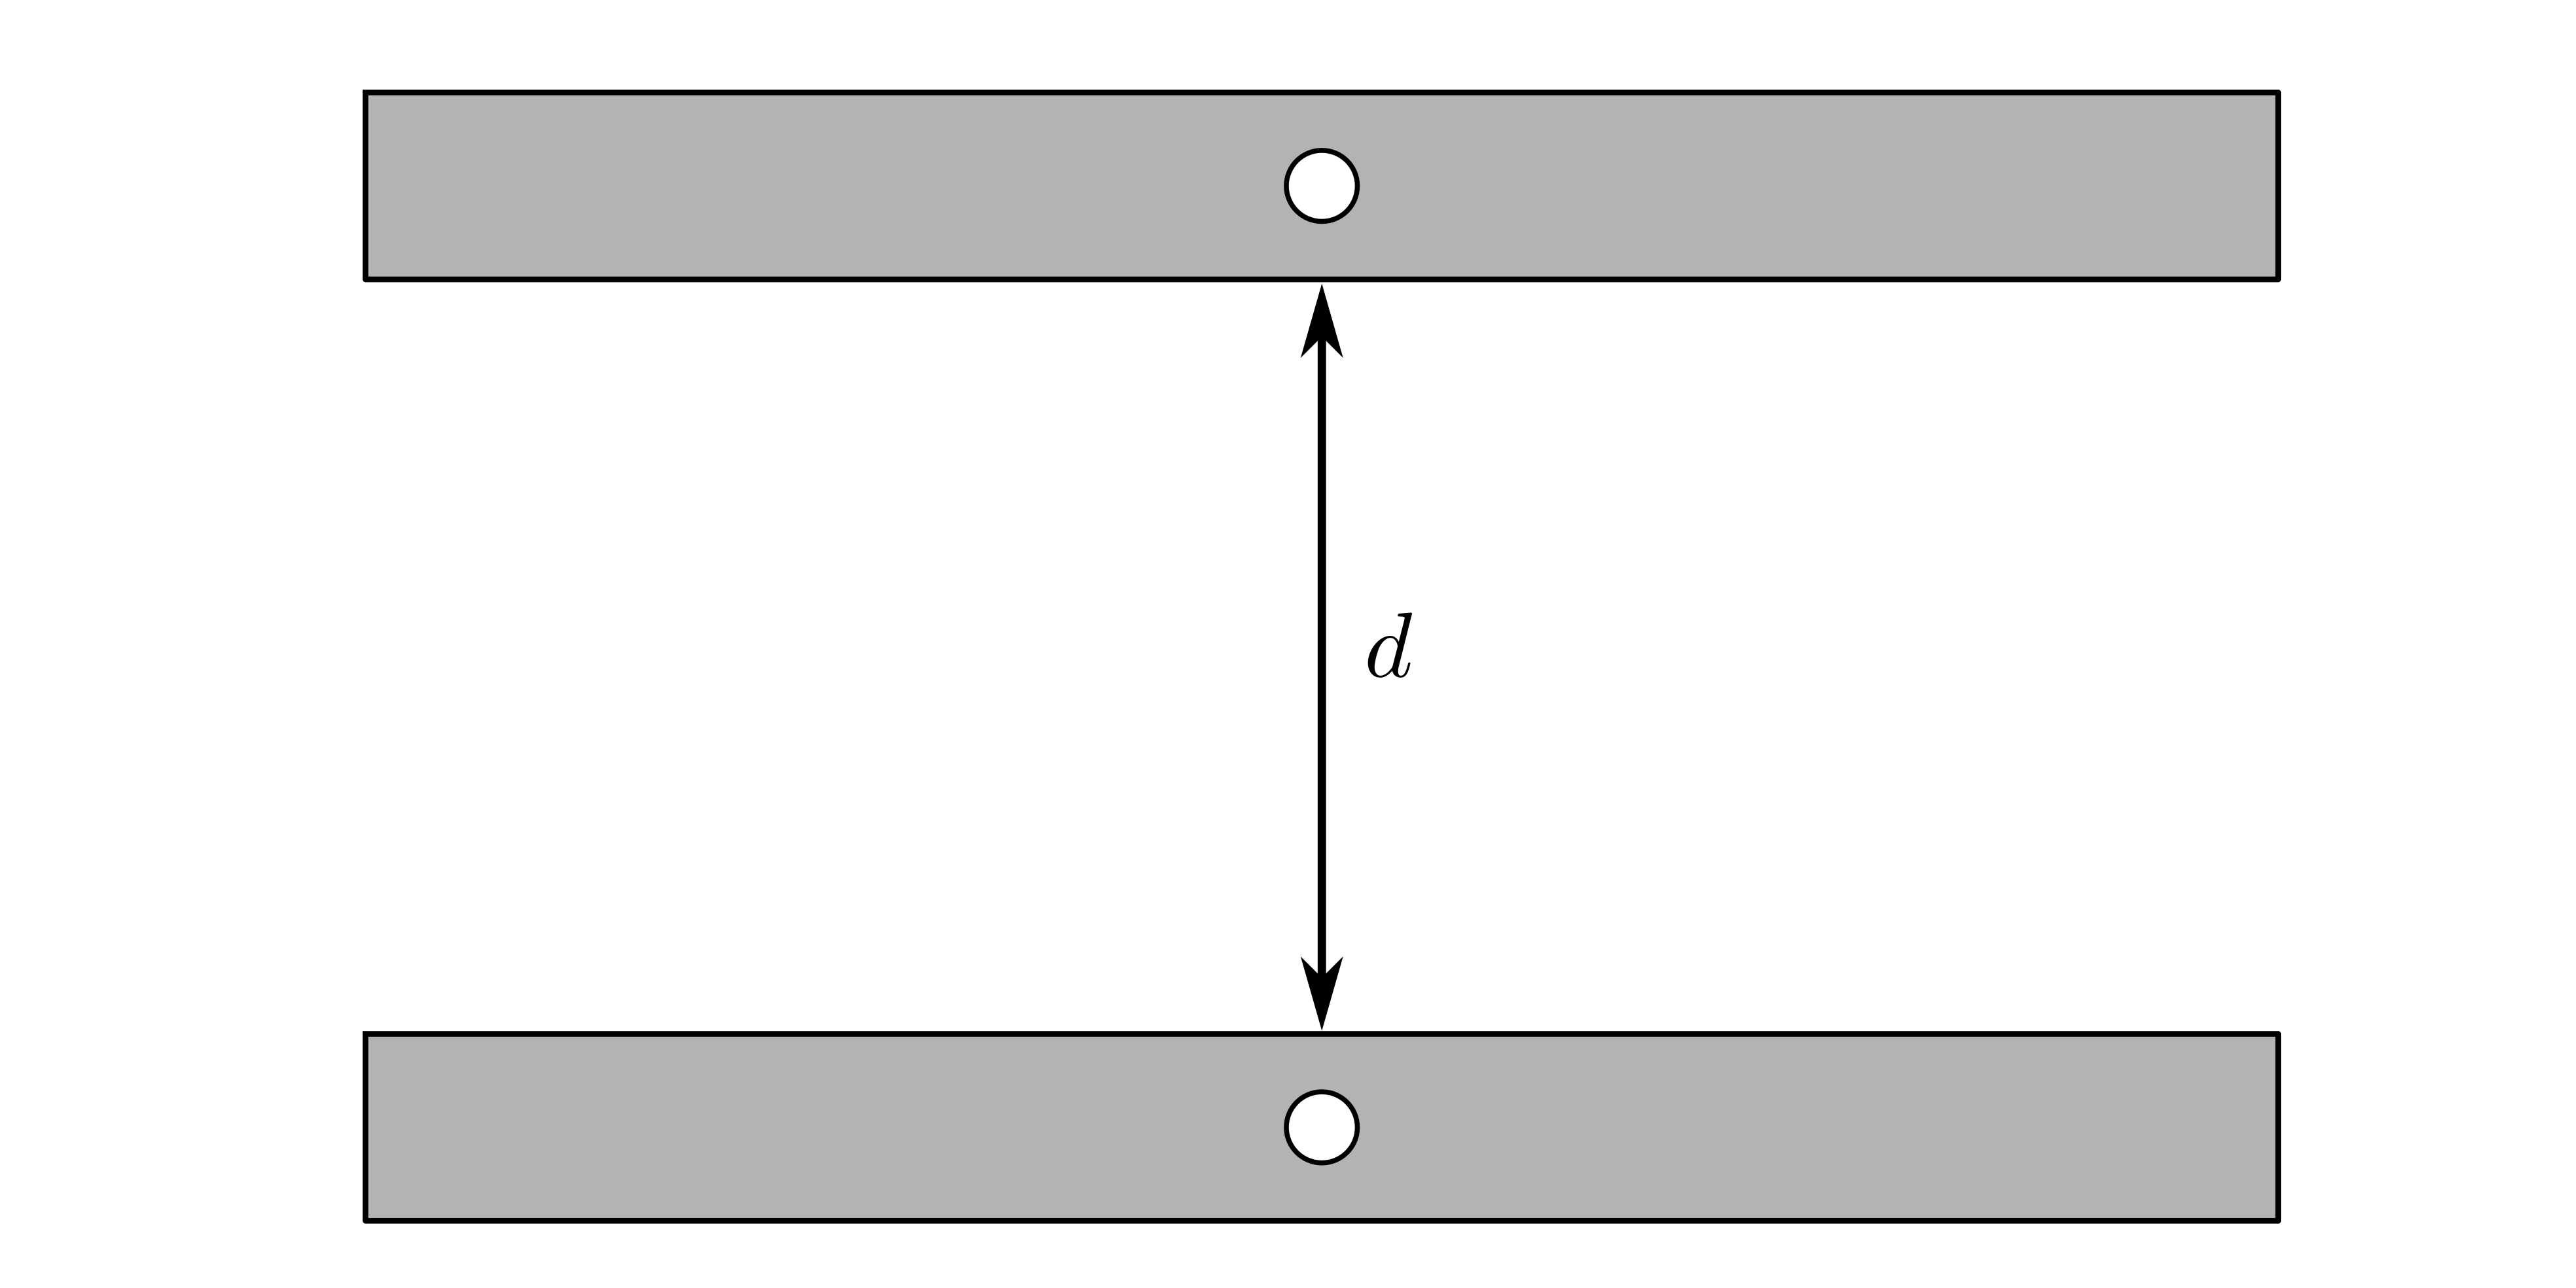
\includegraphics[scale=0.5]{figs/equipotential-curves/equipotential-parallel-plates.png}
                \caption{ ``Infinite" parallel bars}
                \label{fig:parallel-plates}
        \end{subfigure}\hfill
        \begin{subfigure}[b]{0.4\textwidth}
        \centering
                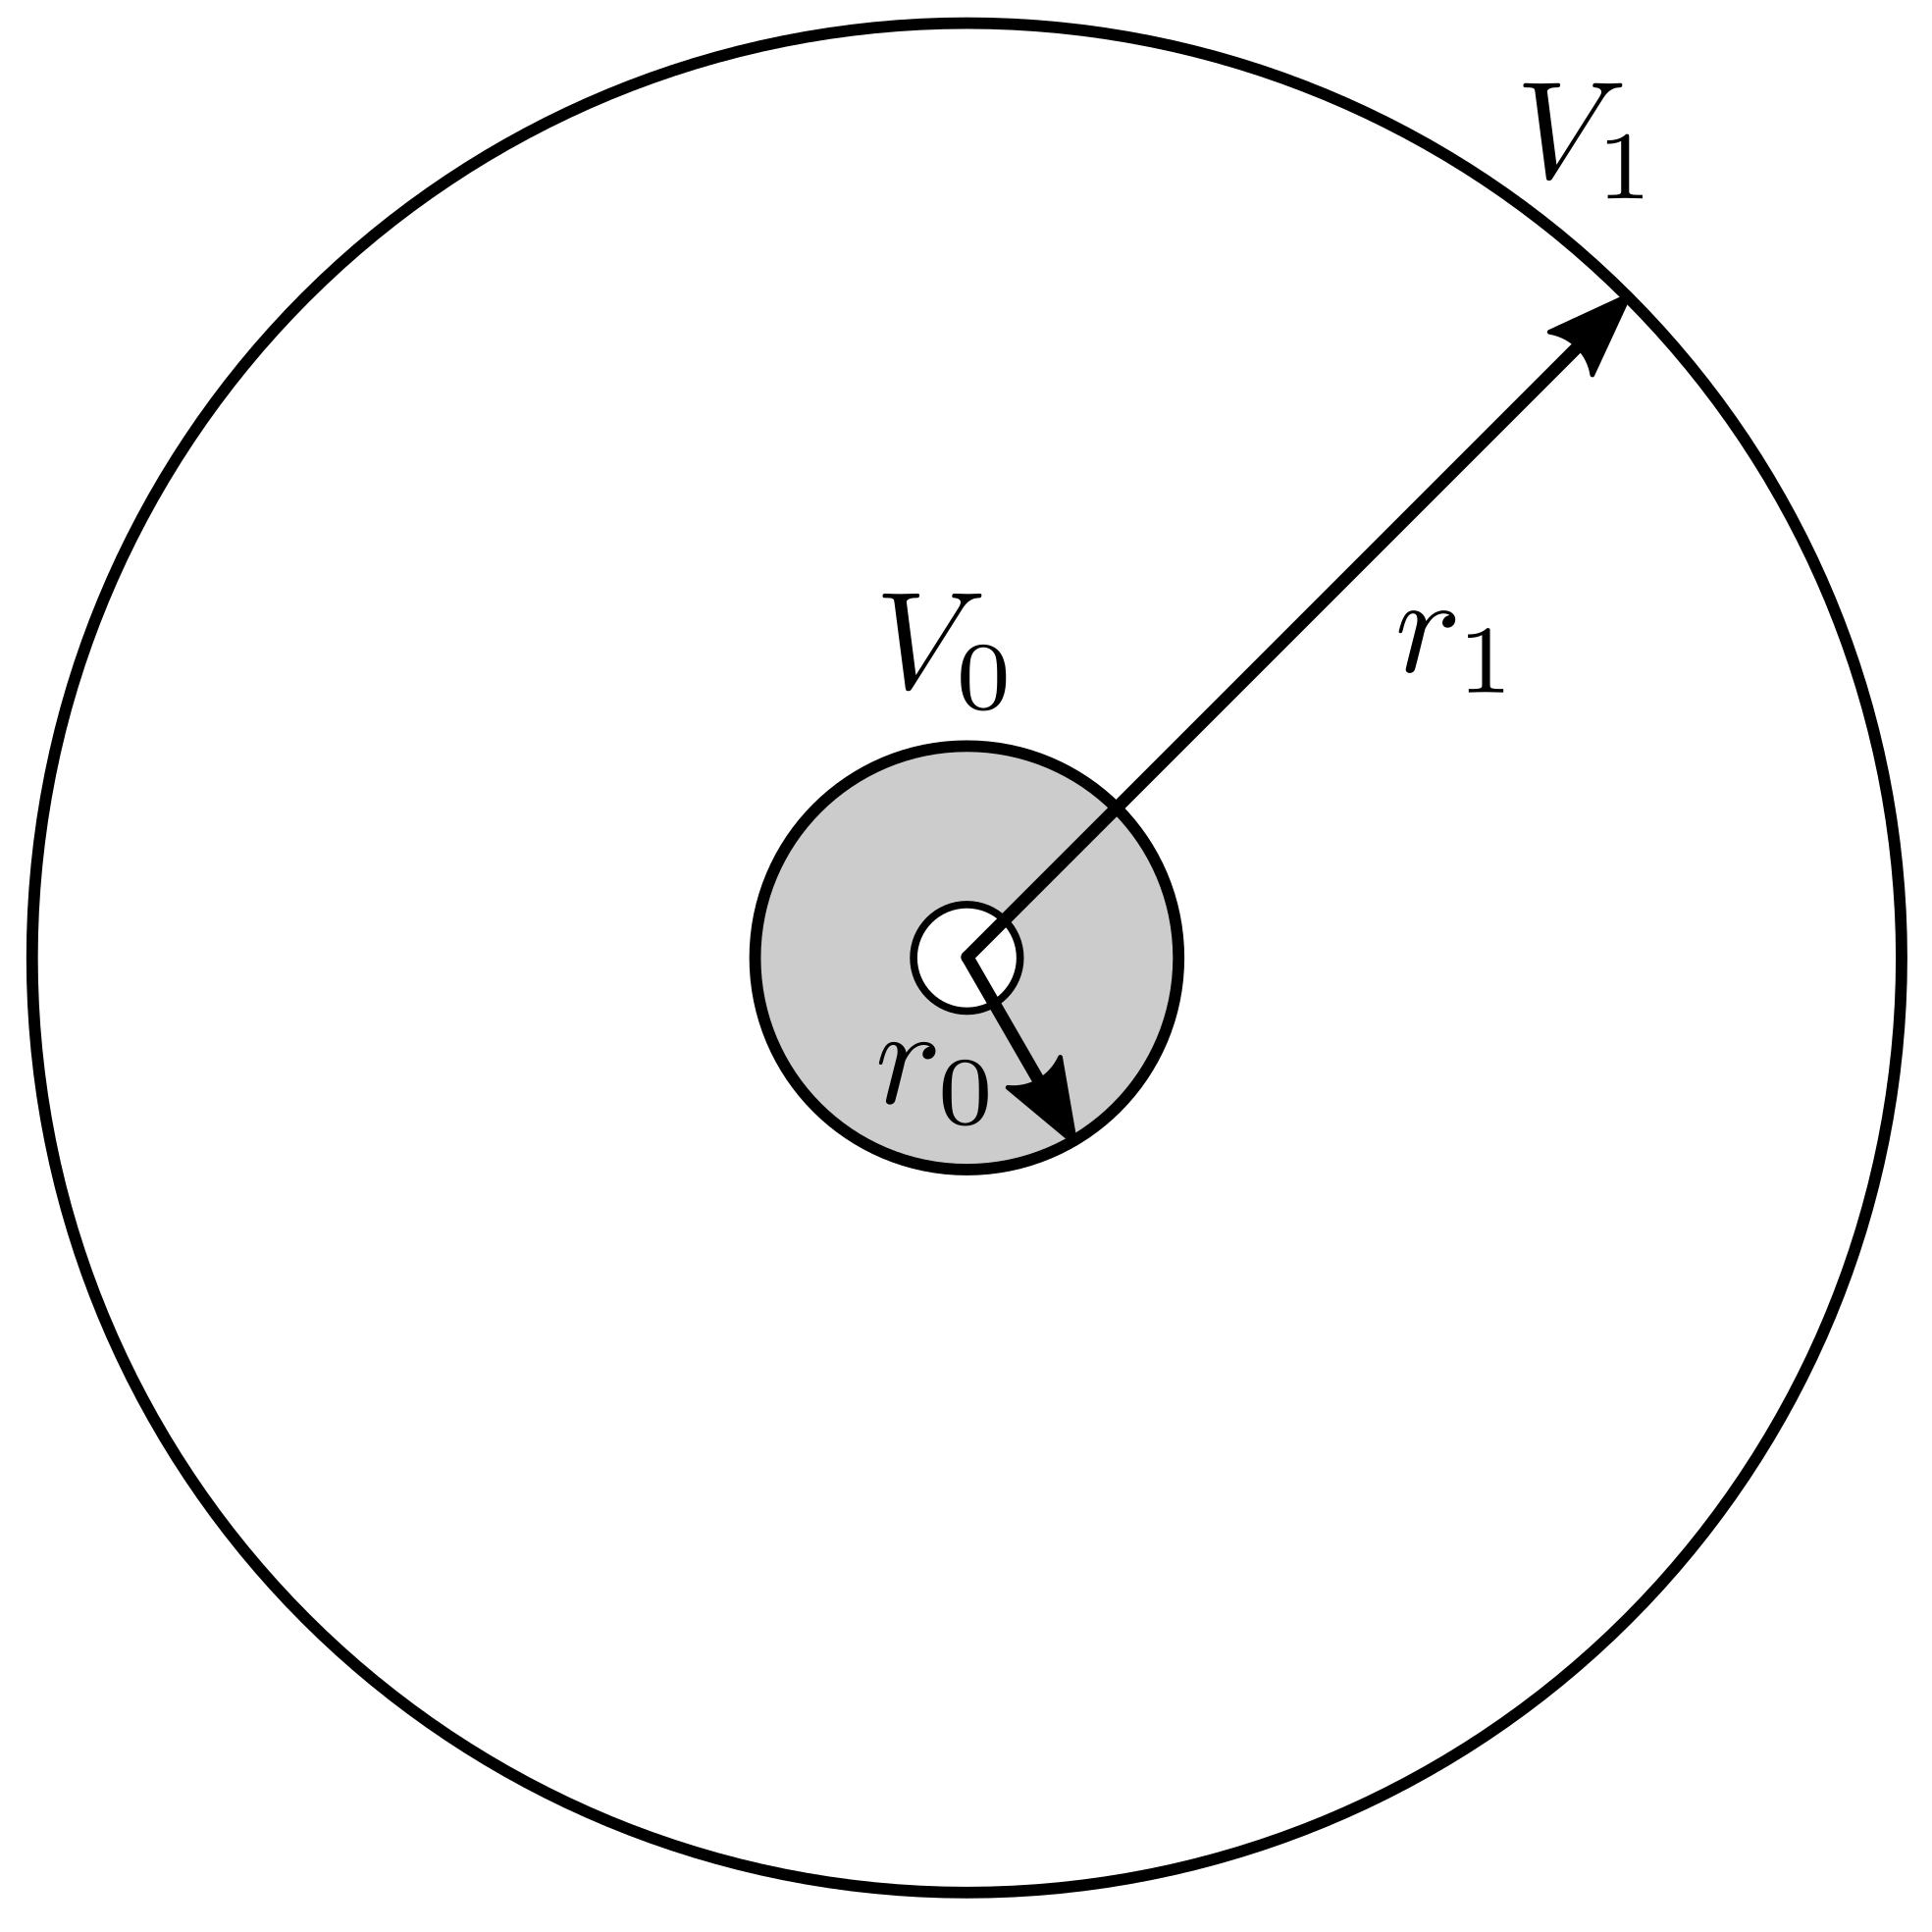
\includegraphics[scale=0.5]{figs/equipotential-curves/equipotential-concentric-cylinders.png}
                \caption{Concentric cylinders}
                \label{fig:concentric-cylinders}
        \end{subfigure}
        \caption{Two exactly solvable electrostatic configurations showing different symmetries.}
        \par\bigskip
\end{figure}


\subsubsection*{The parallel-bar ``capacitor''}

Consider first two parallel bars as shown in Figure~(\ref{fig:parallel-plates}), infinite in one direction and separated by some distance $d$ in the other. Laplace's equation can be written in Cartesian coordinates as
\begin{equation}
    \pdv[2]{V}{x}+\pdv[2]{V}{y} = 0.
\end{equation}

However, since the bars are infinitely long, it should be clear to you that there can be no variation in the potential along $x$ (as the plates are infinite, moving a finite distance to the right or left would not change anything). Thus, the equation reduces to 
\begin{equation}
    \dv[2]{V}{y}= 0.
\end{equation}

\begin{question}
\textbf{Question:} Suppose the top bar is at some potential $V_0$ and the other is grounded (i.e.\ at potential $0$), and they are both separated by some distance $d$. Show that the solution to this equation is
\begin{equation}
    V(y) = V_0 \times \left(\frac{y}{d}\right),
    \label{eqn:parallel-plate-field}
\end{equation}
where $y$ is the distance measured from the bottom bar.
\end{question}


\subsubsection{Two concentric cylinders}

Consider now that you have two concentric cylinders, as shown in Figure~(\ref{fig:concentric-cylinders}) The inner cylinder (of radius $r_0$) is at some potential $V_0$ and the outer cylinder (of radius $r_1$) is grounded. In this case, given the cylindrical symmetry of the problem, it is better to solve the problem in cylindrical coordinates. You can easily show that Laplace's equation can be written as 
\begin{equation}
    \frac{1}{r}\pdv{}{r}\left(r \pdv{V}{r}\right) + \frac{1}{r^2}\pdv[2]{V}{\theta} = 0.
\end{equation}

Just as before, we can ignore the $\theta$ term by symmetry (if we rotate the system by any angle, nothing seems to change). i.e.\ 
\begin{equation}
    \frac{1}{r}\dv{}{r}\left(r \dv{V}{r}\right) =0.
\end{equation}

\begin{question}
\textbf{Question:} Show in this case that Laplace's equation is satisfied by a function of the form
\begin{equation}
V(r) = a \ln\left(\frac{r}{r_0}\right) + b.
\end{equation}

\textbf{Question:} By using the fact that at $r = r_0$, the voltage is $V = V_0$, and when $r = r_1  \neq r_0$, the voltage is $V = V_1$, show that
\begin{equation}
    V(r) = \dfrac{(V_1 - V_0) \ln{\left(\dfrac{r}{r_0}\right)}}{\ln{\left(\dfrac{r_1}{r_0}\right)}}  + V_0.
    \label{eqn:concentric-cylinder-field}
\end{equation}

\end{question}

\section*{Experimental Setup}

\subsection*{Apparatus}

\begin{enumerate}[label=\arabic*)]
\itemsep0em
\item An acrylic tray with electrolytic medium (water)
\item An AC power supply with a voltage stabiliser 
\item A set of metallic electrodes
\item A digital multimeter
\item A pointed probe attached to an $XY-$stage
\item A set of connecting cords
\item A set of measuring scales
\end{enumerate}

 \subsection*{Description}

In this experiment you will study the electric potential produced by sets of metallic electrodes of different shapes and sizes, held at a fixed voltage. To plot the equipotential curves, the metallic electrodes are kept in an acrylic tray such that three-fourths of their height is submersed within an electrolyte (tap-water will do) which is used as an electrolytic tank. An AC potential difference is maintained between the electrodes, which causes a distribution of potential in the electrolyte. By measuring the potentials at different points, one can identify the coordinates of the points of equal potential and consequently plot the equipotential curves on a graph sheet. 

\begin{tip}
This experiment can be performed either with AC or DC voltage from the provided power supply. However, while using DC voltage, electrolysis is found to occur, and the aluminium electrodes begin to get eaten away. As a result, it is advisable to use AC voltage from the power supply.
\end{tip}

\subsection*{Precautions}

\begin{itemize}
\item Arrange the electrodes and keep them stable and undisturbed throughout the measurements. You can use some tape to keep them fixed.
\item Make sure the uninsulated tip of the measuring probe just grazes the surface of the water.
\item Both graph papers -- the one attached below the tray and the one used for noting your data -- should have same coordinates and precision in scale.
\end{itemize}


\section*{Procedure}

Begin by taking two graph sheets and drawing the same coordinate system on them. You will stick one of these sheets on the bottom of the acrylic tray and use it as a reference. You will then mark out the potentials at different points on the other sheet, using the first as a reference.

\subsection*{Part A} 

\begin{enumerate}
    \item Place the two long electrodes parallel to the $x$-axis symmetrically about the origin, as shown in Figure~(\ref{fig:parallel-plates}).
    
    \item A potential difference is established across the electrodes by connecting them to the AC power supply.
    
    \item Using the multimeter, test the potential difference between the electrodes in volts. If it is found to be significantly different from the value you are supplying, ask a TF or instructor for help. 
    
    \begin{question}
        \textbf{Question:} What should the equipotential surfaces look like in this case?
    \end{question}
    
    \item Using the same ground as a reference, connect the positive wire of the multimeter to the probe and qualitatively measure the change in the potential from one end of the acrylic tray to the other.
    
    \item Measure the voltage at an arbitrary point and then find multiple points with the same potential thus drawing out one of the equipotential curves. 
    
    \item Choosing an appropriate increment in voltage, find the equipotential curves for different values of the potential. Verify Equation~(\ref{eqn:parallel-plate-field}) in the appropriate limit. 
    
    \begin{question}
        \textbf{Question:} Do you see Equation~(\ref{eqn:parallel-plate-field}) being satisfied everywhere? What could be the reason for this?
    \end{question}


\end{enumerate}


\subsection*{Part B}

\begin{enumerate}
    \item Set up the electrodes as shown in Figure~(\ref{fig:concentric-cylinders}). Maintain the inner cylinder at a higher voltage $V_0$ and ground the outer cylinder.
    
    \begin{question}
        \textbf{Question:} What should the equipotential surfaces look like in this case?
    \end{question}
    
    \item As before, choose an appropriate increment in voltage and find the equipotential curves for different values of the potential. 
    
    \item Use this to verify the equation for the voltage between two concentric cylinders, given in Equation~(\ref{eqn:concentric-cylinder-field}).
\end{enumerate}



\subsection*{Part C}

Explore the equipotential curves for a single configuration of your choice. 

\begin{tip}
    You can visit following online applet: \nolinkurl{falstad.com/emstatic/} and play around with the various different configurations to see how the field lines and contour lines are produced by different distributions of charges. 
\end{tip}